\chapter{DEPLOYMENT}

\section{Deployment Architecture}

\begin{figure}[H]
\centering
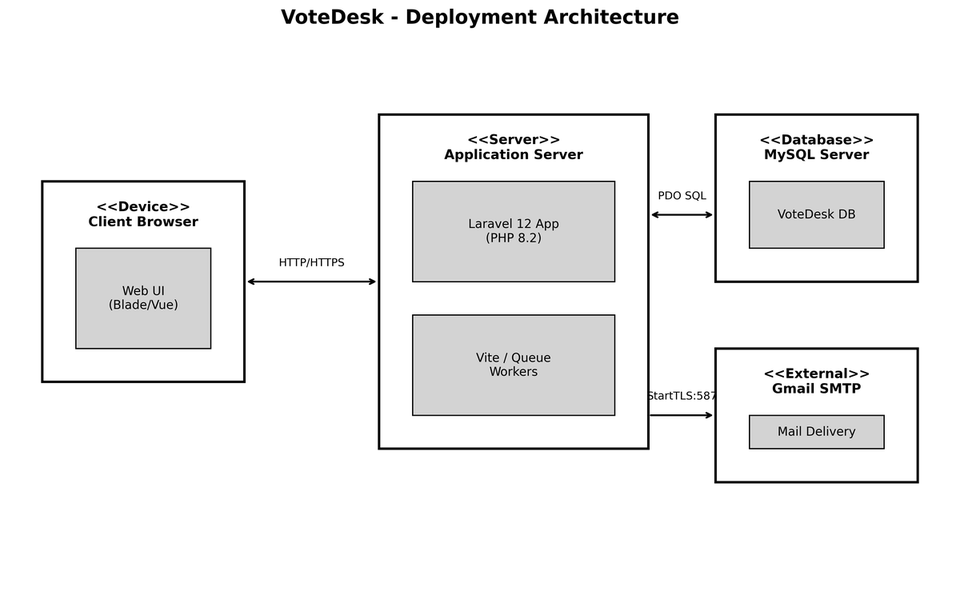
\includegraphics[width=\textwidth,height=0.75\textheight,keepaspectratio]{deployment_architecture.png}
\caption{VoteDesk Deployment Architecture Diagram}
\label{fig:deployment}
\end{figure}

The deployment architecture diagram illustrates the hardware and software nodes required to host the digital election system.

\section{Folder Structure}

The VoteDesk application follows the standard Laravel project directory structure, which promotes modularity, separation of concerns, and maintainability. The key directories are described below.

\subsection*{Main Project Directories}

\textbf{app/} \\
The core application directory, organised as follows:
\begin{itemize}
    \item \texttt{Http/Controllers/} -- Contains all eight controllers: \texttt{AuthController}, \texttt{RegistrationController}, \texttt{AdminController}, \texttt{BLOController}, \texttt{VoterController}, \texttt{CandidateController}, \texttt{ElectionController}, and \texttt{ForgotPasswordController}.
    \item \texttt{Http/Middleware/} -- Contains \texttt{RoleMiddleware}, which enforces role-based access control on all protected routes.
    \item \texttt{Models/} -- Contains Eloquent models: \texttt{User}, \texttt{Voter}, \texttt{Candidate}, \texttt{BLO}, \texttt{Panchayat}, \texttt{Vote}, and \texttt{ElectionConfig}.
    \item \texttt{Mail/} -- Contains mail classes: \texttt{OtpMail} and \texttt{CandidateApprovedMail}.
\end{itemize}

\textbf{routes/} \\
The \texttt{web.php} file defines all application routes, grouped by middleware. Public routes include registration, login, and candidate application. Protected routes are grouped under the \texttt{auth} middleware and further sub-grouped under \texttt{role} middleware for \texttt{voter}, \texttt{blo}, \texttt{admin}, and \texttt{candidate} roles.

\textbf{resources/} \\
Contains all frontend assets:
\begin{itemize}
    \item \texttt{views/} -- Blade templates organised into sub-folders: \texttt{admin/}, \texttt{blo/}, \texttt{voter/}, \texttt{candidate/}, \texttt{auth/}, \texttt{election/}, \texttt{emails/}, and \texttt{layouts/}.
    \item \texttt{css/app.css} and \texttt{js/app.js} -- Frontend entry points processed by Vite.
\end{itemize}

\textbf{database/} \\
Contains:
\begin{itemize}
    \item \texttt{migrations/} -- 19 migration files that define the full database schema and all incremental schema changes.
    \item \texttt{seeders/DatabaseSeeder.php} -- Seeds three default panchayats, an admin user, and the initial ElectionConfig record.
\end{itemize}

\textbf{public/} \\
The web server document root. Contains \texttt{index.php} (the Laravel entry point), compiled frontend assets, and the symlinked \texttt{storage/} directory for user-uploaded and captured files.

\textbf{storage/} \\
Stores application-generated files, including voter verification photos (\texttt{voter\_photos/}) and candidate profile photos (\texttt{candidate\_photos/}).

\textbf{config/} \\
Contains configuration files for database (\texttt{database.php}), mail (\texttt{mail.php}), filesystem (\texttt{filesystems.php}), authentication (\texttt{auth.php}), and session (\texttt{session.php}).

\section{Environment Setup}

Before running the application, the following software must be installed:

\begin{itemize}
    \item PHP 8.2 or higher (with extensions: \texttt{pdo\_mysql}, \texttt{mbstring}, \texttt{openssl}, \texttt{fileinfo})
    \item Composer (PHP dependency manager)
    \item MySQL 8.0 or higher
    \item Node.js 18+ and NPM
    \item Git
\end{itemize}

Configure the \texttt{.env} file with the following key values:

\renewcommand{\arraystretch}{1.3}
\begin{table}[H]
\centering
\begin{tabular}{|p{5cm}|p{7cm}|}
\hline
\textbf{Environment Variable} & \textbf{Description} \\
\hline
\texttt{APP\_NAME} & VoteDesk \\
\hline
\texttt{DB\_HOST} & MySQL server host (e.g., 127.0.0.1) \\
\hline
\texttt{DB\_PORT} & MySQL port (default: 3306) \\
\hline
\texttt{DB\_DATABASE} & Database name (e.g., election\_system) \\
\hline
\texttt{DB\_USERNAME} & MySQL username \\
\hline
\texttt{DB\_PASSWORD} & MySQL password \\
\hline
\texttt{MAIL\_MAILER} & smtp \\
\hline
\texttt{MAIL\_HOST} & smtp.gmail.com \\
\hline
\texttt{MAIL\_PORT} & 587 \\
\hline
\texttt{MAIL\_USERNAME} & Gmail address for OTP sending \\
\hline
\texttt{MAIL\_PASSWORD} & Gmail App Password \\
\hline
\end{tabular}
\caption{Key Environment Configuration Variables}
\label{tab:env_config}
\end{table}

\section{Installation}

Follow these steps to set up and run the VoteDesk system:

\begin{enumerate}
    \item \textbf{Clone or extract the project} into your desired directory.
    \item \textbf{Install PHP dependencies:}
    \begin{verbatim}
    composer install
    \end{verbatim}
    \item \textbf{Copy and configure the environment file:}
    \begin{verbatim}
    copy .env.example .env
    \end{verbatim}
    Then edit \texttt{.env} with your database and mail credentials.
    \item \textbf{Generate the application key:}
    \begin{verbatim}
    php artisan key:generate
    \end{verbatim}
    \item \textbf{Run database migrations and seed default data:}
    \begin{verbatim}
    php artisan migrate --seed
    \end{verbatim}
    \item \textbf{Create the storage symbolic link} (for serving uploaded files):
    \begin{verbatim}
    php artisan storage:link
    \end{verbatim}
    \item \textbf{Install frontend dependencies:}
    \begin{verbatim}
    npm install
    \end{verbatim}
    \item \textbf{Build frontend assets:}
    \begin{verbatim}
    npm run build
    \end{verbatim}
\end{enumerate}

\section{Running the System}

To start the development server:

\begin{verbatim}
php artisan serve
\end{verbatim}

The application will be accessible at \texttt{http://localhost:8000}.

Optionally, to run all services concurrently (server, queue worker, and Vite dev server):

\begin{verbatim}
composer run dev
\end{verbatim}

The default administrator account created by the seeder has the following credentials:

\begin{itemize}
    \item \textbf{Email:} admin@example.com
    \item \textbf{Password:} password
\end{itemize}

It is strongly recommended to change these credentials immediately in a production environment.
